\chapter{Conclusion}
\label{chap: Chapter 8}

Based on the discussion in the previous chapter, it is clear that using various Natural Language Processing and text mining techniques outlined in chapter \ref{chap: Chapter 6} would indeed be possible.
It was apparent that adjusting the parameters of the prototype also played a major part in the quality of the topics. Later such topics directly influenced the recommendation list.

This chapter provides a summary of the study to conclude the study findings. The next section will discuss how the research objectives were reached. After the section of how the research objectives were accomplished, suggestions for future research will be made.

\section{Revisiting the research objectives}

This section facilitates a discussion on how the research objectives were met. As mentioned in chapter 1, the primary research objective was to \textbf{\textit{Develop a model to recommend related research papers.}}

Achieving the primary objective depended on meeting the secondary objectives listed in Chapter \ref{chap: Chapter 1}.

\textbf{SO 1}: \textit{To identify recommender systems techniques and how they are used.}

This secondary objective was met by surveying the literature of Recommender Systems. As this secondary objective's goal was to map and understand what techniques are used in recommender systems and how researchers utilise it. I looked at the various approaches that not only fits the use case of the study but also which is relevant. It was decided that the Content Based Filtering approach would the best to use since no assumptions are made of users activity. In addition to this, CBF does not care about user ratings, it looks at the content of the documents. It was critical to look for approaches that does not rely on user activity and user ratings. Chapter \ref{chap: Chapter 2} was dedicated to introduce the concepts of how modern Information Systems (Recommender Systems) work and how they evolved from the past to recent years. A continuation on the introduction to the fields was found in Chapter \ref{chap: Chapter 3}.

\textbf{SO 2}: \textit{To identify machine learning techniques that assist with the recommender task.}

This secondary objective was met by surveying several machine learning techniques. The goal of this objective was to identify and better understand what machine learning techniques there are, and how they tie into recommender type systems.
Machine Learning in section \ref{ssec:MLoverview}, Natural Language Processing in section \ref{secc:LDAover} and Topic Modeling in section \ref{ssec:tmodel} paved the way to understand the technology that would be used in this study.

The selection of the topic model algorithm that would be most suitable was also stemmed from literature. More specifically in section \ref{ssec:tmodel} it was discussed that Latent Dirichlet Allocation (LDA) was a very popular choice for building such topic models. Furthermore, section \ref{ssec:LDAA} explains how LDA works, by computing hidden topic structures from documents.

Before developing the conceptual model, the research methodology was discussed in Chapter \ref{chap: Chapter 4}. More specifically the research process that will be followed to conceptualise the model based on the previous chapters

Formulating the concepts into a plan of action, Chapter \ref{chap: Chapter 5} was introduced. The conceptual model was developed by looking at content covered in Chapters \ref{chap: Chapter 2} and \ref{chap: Chapter 3}. The Data Analytics lifecycle was adopted as seen in Figure \ref{fig:lifecycle} to help conceptualise the model.

Chapter \ref{chap: Chapter 6} was crucial to better understand the concepts introduced by Chapters Chapter \ref{chap: Chapter 2} and Chapter \ref{chap: Chapter 3}. The prototype served as dual purpose. The prototype highlighted parameters that has an influence on the prototype but also the overarching model. In addition to this, building a prototype using concepts in the other chapters helped the model proved that the model is feasible. Using information security research papers with security specific wording also proved the model to be applicable to domains like information security.

Throughout the prototype and model development, practical lessons were learned. Those reflections 
were shared in Chapter \ref{chap: Chapter 7}. Especially, looking at Figure \ref{fig:processing1}, we can see which lessons were learned for each phase of the conceptual model.

In the next section, we discussed the proposed model.

\section{The Proposed Model}

\begin{figure}[htbp]
\centering
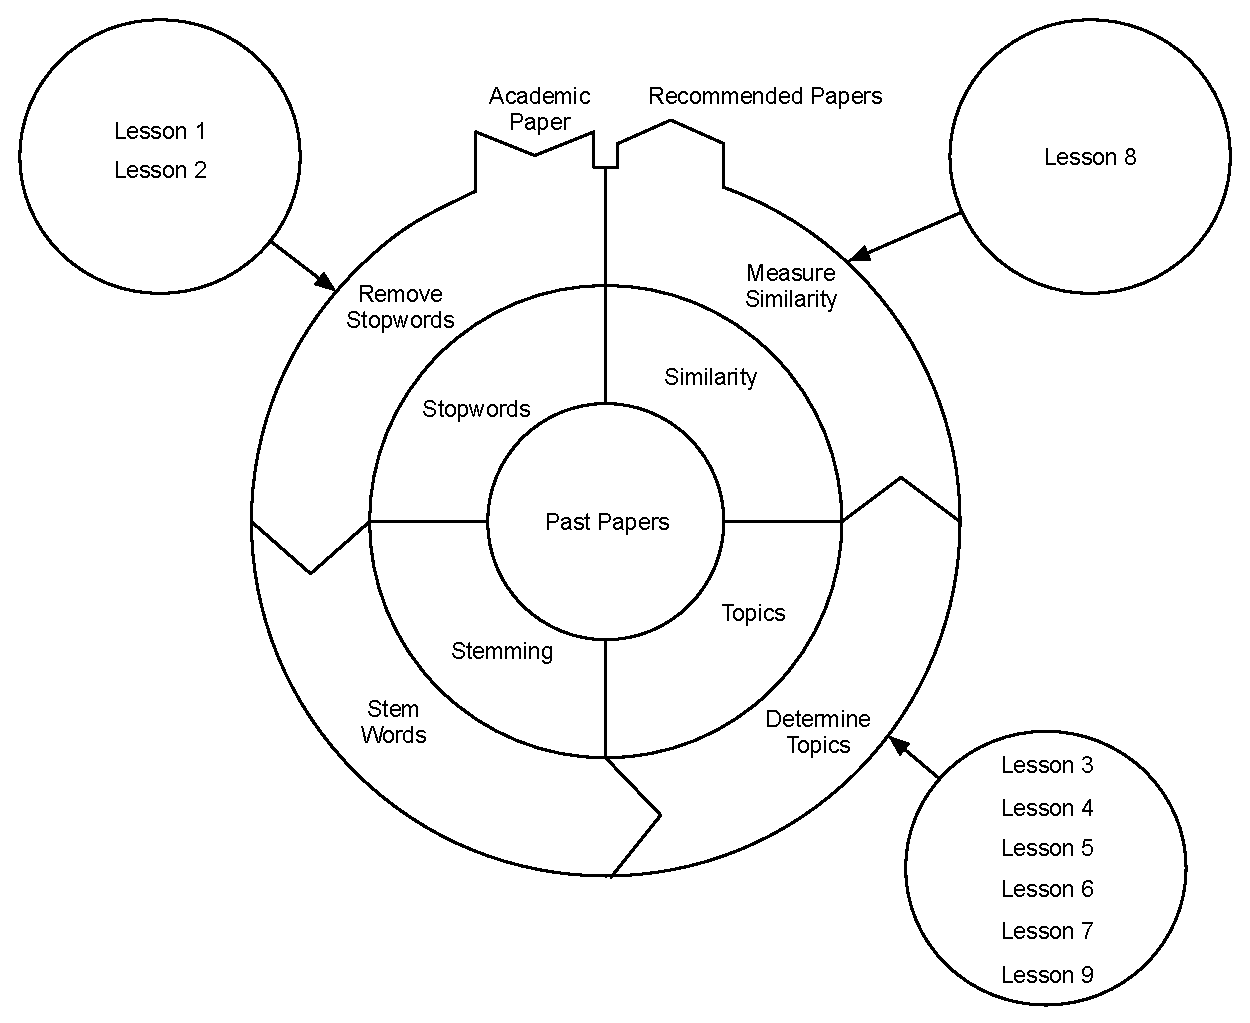
\includegraphics[width=15cm]{./figures/Lesson.eps}
\caption{Mapping lessons learned to the model}
\label{fig:processing1}
\end{figure}

This section discusses the proposed model of this study, which met the primary research objective \textbf{\textit{To develop an Recommender system which will automatically recommend similar research papers.}}

The content in chapters \ref{chap: Chapter 2} and \ref{chap: Chapter 3} set the foundation for the rest of the study. Moreover, Chapter \ref{chap: Chapter 2} focused on recommender systems, what the recommendation task entails and what the different types of recommender systems exist. 

Chapter \ref{chap: Chapter 3} explored the different machine learning technologies which are linked to recommender systems. Looking at the data that was used, the data was not labeled. As guided by literature, the suggested approach was to use unsupervised learning, to look for underlying themes. Furthermore, to help identify underlying themes document clustering which is a subset of machine learning was used in the prototype. Having two or more probability distributions, the similarity between the distributions was identified.

The suggested algorithms and processes in the previous chapters greatly influenced the research design chapter. As this study finds itself in the exploratory sphere, it was important to understand the research paradigm. Understanding the paradigm led to choosing a set of research methods and therefore, a plan of action on how to achieve the research goals.

The conceptual model was created using literature from Chapters \ref{chap: Chapter 2} and \ref{chap: Chapter 3} and guided by Chapter \ref{chap: Chapter 4}. The conceptual model, in Chapter \ref{chap: Chapter 4}, used the Data Analytics Lifecycle and adapted to the use case of this study. A prototype was developed to help the researcher understand how all these concepts fit together.

The prototype was developed with dual purpose and was documented in Chapter \ref{chap: Chapter 6}. The prototype provided the ability to observe the influence parameters has on recommendations. The experiments were conducted and documented in Chapter \ref{chap: Chapter 7}. The other purpose was to check if the model and prototype is feasible and applicable. The researcher used technologies which are still relevant today. Using these technologies and real conference data to test the prototype deems this study feasible and applicable.

Lastly, Chapter \ref{chap: Chapter 7} hosted the discussion to what practical lessons were learned during the development of the prototype, as seen in Figure \ref{fig:processing1}. 

In summary, Figure \ref{fig:processing1} represents the collection of work done in Chapters \ref{chap: Chapter 5}, \ref{chap: Chapter 6} and \ref{chap: Chapter 7}. After constructing the conceptual model in Chapter \ref{chap: Chapter 5} based on literature, chapter \ref{chap: Chapter 6} focused on validating the conceptual model. The validation was done by developing a prototype which was outlined in \ref{chap: Chapter 6}. Lastly, chapter \ref{chap: Chapter 7} included all the lessons that was learned throughout the process constructing the model and developing the prototype.

In the next section, research limitations will be discussed.

\section{Research Limitations}
This study has some limitations that must be recognized. The first limitation is that of the sample size. At the time of data collection, the information security South Africa conference only had 254 research papers to use in the dataset. Of that 254 research papers certain topics are discussed in a small number. If the topics are scarce during training, the recommendation task will be very difficult to complete. The goal was to train and test the prototype using one specific library of one conference.

The second limitation is that only one topic modeling technique (Latent Dirichlet Allocation) was used. There were several reasons behind it namely, recent research suggested that when using Content-based approaches, Latent Dirichlet Allocation would be preferred. 
Considering time constraints as this is a Masters study, we felt to go ahead with the one topic modeling technique.

The third limitation, this study only uses Jensen-Shannon Divergence to calculate the similarity between the two data spaces (Test set and training set). Similar to the second limitation, time did not allow us to venture deeper into different similarity measures.

Lastly, the forth limitation includes not having a human factor to evaluate each phase individually. The phases which are referred to is the outputs of the Topic Modeling technique and, also the end result of the similarity measurement. 

\section{Suggestions for further research}
This section is dedicated to outline further research to be done on the limitations which was raised in the previous section. Future research could possibly be conducted using a conference that has more research papers to their disposal. It will provide more data to be clustered and ultimately better the similarity measures. This relates to the first limitation.

Reflecting on the second limitation, the study could include multiple Topics Modeling algorithms and compare the outputs. Algorithms like Non Negative Matrix Factorization (NMF) \cite{Purpura2018}, Latent Semantic Analysis (LSA) \cite{Qomariyah2019}, Parallel Latent Dirichlet Allocation (PLDA) \cite{Mukherjee2019} and Pachinko Allocation Model (PAM) \cite{Koltcov2021}. 

Similarly, the third limitation, using different similarity measures could lead to different recommendations. Furthermore, mixing different Topic Models with similarity measures could yield better results.

The forth limitation which includes human intervention to evaluate each phase could sped up the model implementation, since getting feedback every step of the way.

The four limitations can also be seen as practical lessons that the researcher has learned. Along with the Table \ref{tab:lessons}, suggestions for further research and lesson learned can be seen as the same.

\section{Epilogue}
This study identified that it's time consuming for researchers to look for related research papers. This problem was addressed by developing a model to recommend related research papers. During the development of the model and prototype, it was evident that machine learning bridges the gap of spotting latent themes. However, the lessons learned Chapter \ref{chap: Chapter 7}, shows that when other researchers endeavour onto similar topics a great learning curve awaits. The researcher hopes that this study motivates other researchers to advance the natural language processing and machine learning research angle traditional topics.